\chapter{Cosmologie newtonienne et équation de Friedmann}

La dernière fois, nous parlions de la métrique de l’espace. La question suivante porte sur la dynamique : comment le facteur d’échelle évolue-t-il au cours du temps ? Commençons par un peu de géométrie, puis passons à la cosmologie newtonienne. Nous ne dériverons pas encore l’équation de Friedmann à partir de la relativité générale. Nous la dériverons à partir des équations de Newton.

\section{Homogénéité, isotropie et métrique dépendant du temps}

L’homogénéité et l’isotropie sont les hypothèses de départ. Si l’Univers est homogène et isotrope et qu’il évolue au cours du temps, alors la loi de Hubble est toujours vérifiée. À tout instant fixé, la vitesse de récession est proportionnelle à la distance,
\begin{equation}
v = H(t)\,d.
\end{equation}
La proportionnalité est linéaire. Ce qui est constant, ce n’est pas le temps, mais l’espace : à un instant donné, le même coefficient de proportionnalité s’applique partout.

\begin{classroomqa}
\audiencequestion{Cela signifie-t-il que la proportionnalité est linéaire ?}\lecturetimestamp{00:02:06}
\lecturerresponse{Oui. À un instant fixé, la vitesse de récession est linéairement proportionnelle à la distance. Le coefficient de proportionnalité est la constante de Hubble. En général, il dépend du temps, mais il ne varie pas d’un point à l’autre de l’espace.}
\end{classroomqa}

C’est pourquoi l’expression ``constante de Hubble'' peut induire en erreur. Elle est constante par rapport à la position dans l’espace, mais pas par rapport au temps.

Une question naturelle se pose alors. Si l’espace se dilate, pourquoi les règles graduées ne se dilatent-elles pas elles aussi ? Parce qu’elles sont maintenues par des forces immensément plus puissantes que tout effet associé à l’expansion cosmologique à l’échelle atomique. Les objets liés restent liés. Ce sont les distances entre des objets suffisamment éloignés les uns des autres, comme des galaxies trop distantes pour être fortement liées entre elles, qui augmentent.

\begin{classroomqa}
\audiencequestion{La question se pose-t-elle de savoir si les règles de mesure se dilatent elles aussi ?}\lecturetimestamp{00:04:00}
\lecturerresponse{Non. Les règles de mesure ne se dilatent pas. Ce sont les coordonnées qui se dilatent. Les forces qui maintiennent les règles graduées sont bien plus puissantes que les effets de l’expansion ; les objets ordinaires liés ne se dilatent donc pas avec le fond cosmologique. Les galaxies suffisamment éloignées les unes des autres s’écartent, mais pas les règles graduées.}
\end{classroomqa}

On peut même imaginer un minuscule effet répulsif supplémentaire entre les atomes. Cela ne suffirait toujours pas à briser une règle : cela ne ferait que déplacer légèrement la distance d’équilibre, comme une faible force supplémentaire modifie la position d’équilibre d’un ressort rigide.

\begin{classroomqa}
\audiencequestion{Mais on ne peut pas le modéliser comme une force entre des points, n’est-ce pas ? Sinon, il y aurait une accélération.}\lecturetimestamp{00:05:29}
\lecturerresponse{On peut imaginer une faible force supplémentaire entre les atomes, mais si elle est minuscule par rapport aux forces de liaison, elle ne fait que déplacer légèrement la position d’équilibre. L’expansion, à elle seule, ne crée pas de loi de force ordinaire. Certains types d’expansion peuvent être modélisés au moyen d’une force, notamment l’expansion accélérée, mais cette question viendra plus tard.}
\end{classroomqa}

Les coordonnées utiles sont donc celles qui sont attachées à la distribution de matière en expansion. Les galaxies dépourvues de mouvement propre supplémentaire conservent les mêmes coordonnées. Ce qui évolue avec le temps, c’est la relation entre la séparation en coordonnées et la distance physique mesurée en mètres. Cette relation est décrite par le facteur d’échelle \(a(t)\).

Dans un espace plat, la métrique spatiale peut s’écrire
\begin{equation}
ds^2 = a(t)^2\left(dx^2+dy^2+dz^2\right).
\end{equation}
Ici, \(a\) est la distance réelle, mesurée en mètres, entre deux points voisins séparés d’une unité de coordonnée. Si l’Univers se dilate, \(a\) dépend du temps.

Pour passer à l’espace-temps, partons de la forme de la relativité restreinte
\begin{equation}
d\tau^2 = dt^2 - ds^2,
\end{equation}
et substituons-y la métrique spatiale. On obtient
\begin{equation}
d\tau^2 = dt^2 - a(t)^2\left(dx^2+dy^2+dz^2\right).
\end{equation}
Les coefficients ne dépendent pas de la position dans l’espace, mais uniquement du temps. C’est ainsi que l’homogénéité s’exprime dans le langage de la métrique. La métrique diagonale a la forme
\begin{equation}
g_{\mu\nu}=\mathrm{diag}\!\left(1,-a(t)^2,-a(t)^2,-a(t)^2\right).
\end{equation}
\editorialnote{La matrice diagonale complète écrite ici correspond à la description orale du tenseur métrique autour de 00:14:33. Le tableau montre clairement l’élément de ligne, mais la matrice n’y est pas entièrement lisible.}

Il n’y a pas de termes extradiagonaux : ni \(dx\,dy\), ni \(dx\,dt\), ni aucun autre terme mixte. La métrique est presque aussi simple que celle de l’espace-temps plat. Sa particularité est que la relation entre la mesure spatiale et le temps dépend elle-même du temps.

\begin{figure}
\centering
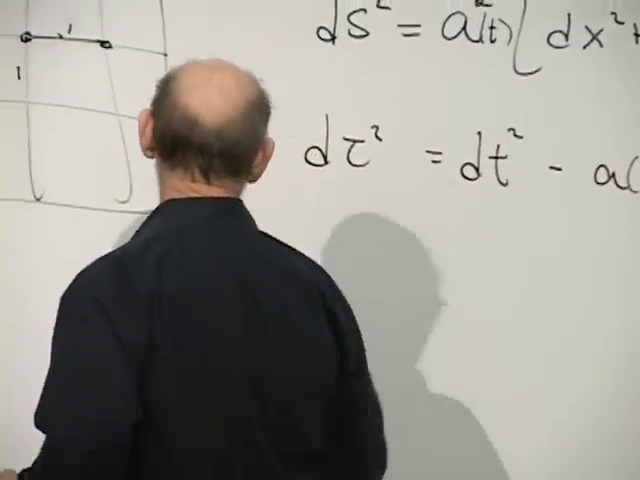
\includegraphics[width=0.62\textwidth]{lecture_02_figure_02.png}
\caption{Schéma d’un réseau comobile et intervalle d’espace-temps avec un facteur d’échelle dépendant du temps.}
\end{figure}

Le schéma illustre l’idée. Alice et Bob restent séparés d’une unité dans les coordonnées comobiles, mais cette unité de coordonnée représente un nombre de mètres toujours plus grand au fil du temps. Si \(a(t)\) était nul à un moment du passé, toute séparation physique serait alors nulle : tout serait écrasé au même endroit. C’est pourquoi \(a\to 0\) correspond à une densité infinie. À mesure que \(a\) augmente, l’Univers devient de plus en plus diffus.

Cette forme de la métrique n’est pas valable dans tous les référentiels. C’est celle du référentiel qui se déplace avec les galaxies.

\begin{classroomqa}
\audiencequestion{Dans cette équation, le petit \(t\), \(a(t)\), à quoi correspond son \(t\) ?}\lecturetimestamp{00:19:19}
\lecturerresponse{C’est le temps mesuré par des horloges qui se déplacent avec les galaxies. Imaginons des horloges identiques, fabriquées dans la même usine d’horloges cosmiques et emportées par les galaxies. Dans ce référentiel, la variable temporelle est précisément ce qu’indiquent ces horloges. Le long de la ligne d’univers d’une galaxie, le temps propre est égal à ce temps coordonnée.}
\end{classroomqa}

En effet, le long de la ligne d’univers d’une galaxie comobile,
\begin{equation}
dx=dy=dz=0,
\end{equation}
donc
\begin{equation}
d\tau^2 = dt^2,
\end{equation}
et par conséquent
\begin{equation}
dt=d\tau.
\end{equation}

\begin{classroomqa}
\audiencequestion{Existe-t-il des transformations qui laissent cette forme de la métrique invariante ?}\lecturetimestamp{00:23:08}
\lecturerresponse{Les rotations, oui, car \(dx^2+dy^2+dz^2\) est invariant par rotation. Les transformations de Lorentz, en revanche, ne préservent pas cette forme. La matière elle-même définit le référentiel qui se déplace avec les galaxies ; dans un autre référentiel, l’Univers ne paraîtrait pas isotrope.}
\end{classroomqa}

\section{Un projectile dans un champ gravitationnel}

Avant d’appliquer les lois de Newton à l’Univers entier, il est utile de revenir à un problème plus simple : une masse importante \(M\), une masse beaucoup plus petite \(m\) et une impulsion initiale vers l’extérieur. Après l’impulsion, la petite masse se déplace simplement dans le champ gravitationnel et suit les lois de Newton.

Pour la discussion cosmologique, le problème complet de l’orbite n’est pas l’essentiel. C’est la conservation de l’énergie qui importe. L’énergie cinétique est
\begin{equation}
\frac{1}{2}mv^2.
\end{equation}

\begin{figure}
\centering
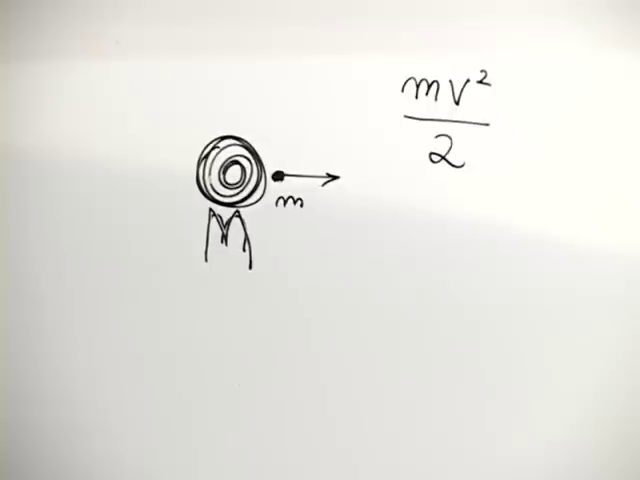
\includegraphics[width=0.42\textwidth]{lecture_02_figure_03.png}
\caption{Masse d’épreuve lancée vers l’extérieur et terme d’énergie cinétique \(\frac{1}{2}mv^2\).}
\end{figure}

L’énergie potentielle gravitationnelle contient le produit des masses et de la constante de Newton, divisé par la distance. Dans l’écriture au tableau, les facteurs apparaissent dans l’ordre \(mMG/D\) ; conservons donc cet ordre ici :
\begin{equation}
-\frac{mMG}{D}.
\end{equation}
L’énergie totale est donc
\begin{equation}
\frac{1}{2}mv^2-\frac{mMG}{D}.
\end{equation}
La conservation de l’énergie signifie simplement que cette quantité ne varie pas au cours du temps pour la particule considérée. Des particules différentes peuvent avoir des énergies différentes.

\begin{figure}
\centering
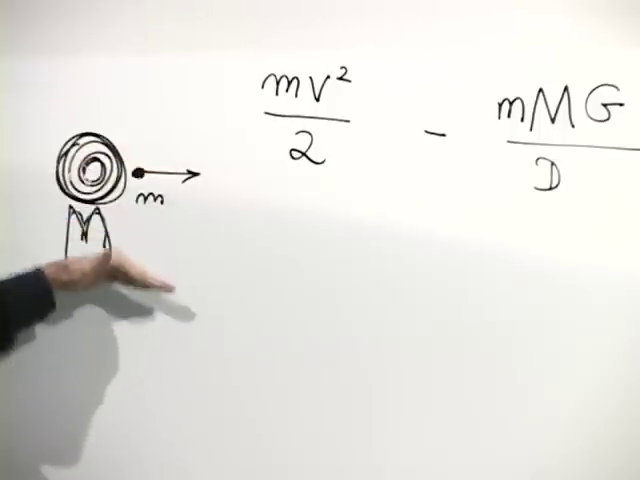
\includegraphics[width=0.62\textwidth]{lecture_02_figure_04.png}
\caption{Énergie totale newtonienne d’une masse d’épreuve en mouvement radial : terme cinétique moins potentiel gravitationnel.}
\end{figure}

Le signe moins est important. L’énergie potentielle gravitationnelle est négative parce que la gravitation est attractive. Quand la particule se rapproche, l’énergie potentielle devient plus négative. Quand elle s’éloigne, elle devient moins négative.

\begin{classroomqa}
\audiencequestion{L’énergie potentielle augmente-t-elle avec la distance plutôt que de diminuer ?}\lecturetimestamp{00:34:13}
\lecturerresponse{Oui. Oublions les constantes et regardons les graphes de \(1/D\) et de \(-1/D\). La force pousse dans le sens d’une diminution de l’énergie potentielle. Une force attractive correspond donc à la courbe inversée, \(-1/D\) : l’énergie potentielle augmente avec la distance et devient plus négative à mesure que la particule se rapproche.}
\end{classroomqa}

\begin{figure}
\centering
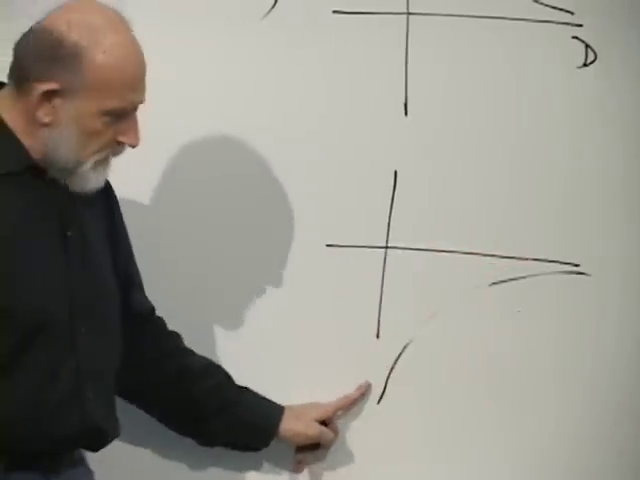
\includegraphics[width=0.46\textwidth]{lecture_02_figure_05.png}
\caption{Comparaison qualitative de \(1/D\) et de \(-1/D\) pour déterminer le signe de l’énergie potentielle gravitationnelle.}
\end{figure}

\section{Vitesse de libération}

Classons maintenant les possibilités. L’énergie peut être positive, négative ou nulle. Ce sont les trois seuls cas.

\begin{itemize}
\item Si l’énergie est négative, la particule est liée. Lancée vers le haut à une vitesse trop faible, elle monte, ralentit, s’arrête puis retombe.
\item Si l’énergie est positive, la particule s’échappe. La gravitation la ralentit d’abord, mais pas assez pour l’arrêter ; elle finit par s’éloigner avec une vitesse asymptotique non nulle vers l’extérieur.
\item Si l’énergie est exactement nulle, la particule a la vitesse de libération. C’est le cas limite entre l’évasion et la capture.
\end{itemize}

Si la vitesse initiale est suffisamment faible, le terme de potentiel domine dès le départ et l’énergie est négative.

\begin{figure}
\centering
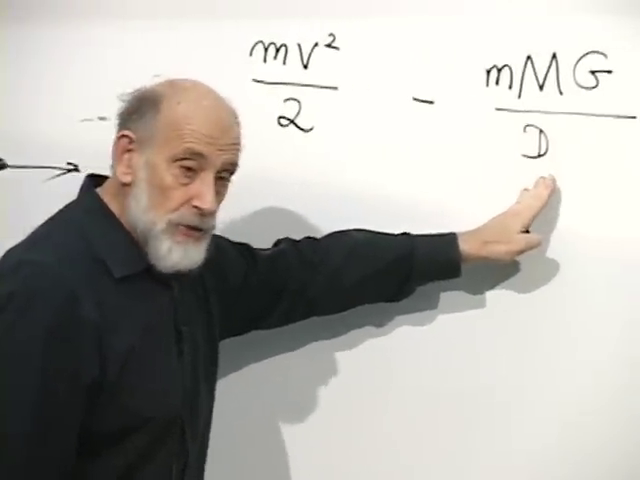
\includegraphics[width=0.62\textwidth]{lecture_02_figure_06.png}
\caption{À faible vitesse vers l’extérieur, le terme de potentiel négatif domine l’énergie totale.}
\end{figure}

Dans le cas d’énergie nulle, la distance continue d’augmenter, tandis que la vitesse diminue. La particule ne peut pas s’immobiliser en un temps fini. Si elle le faisait, elle retomberait. La distance n’est donc pas bornée, tandis que la vitesse tend vers zéro.

C’est l’analogie directe qui importe en cosmologie. L’Univers peut se comporter de la même façon. Si le flot de Hubble initial vers l’extérieur est suffisamment intense, tout s’éloigne de tout le reste. S’il est trop faible, la gravitation l’emporte et l’Univers s’effondre dans un immense écrasement. Il existe aussi un cas limite, exactement analogue à la vitesse de libération.

\section{Théorème de Newton}

La réduction cosmologique fonctionne grâce au théorème de Newton pour la loi en inverse du carré.

Si la matière est distribuée avec une symétrie sphérique autour d’un centre, la force gravitationnelle exercée sur une particule située à l’extérieur de cette distribution est exactement la même que si toute la masse était concentrée au centre. Mais le théorème est plus fort encore. Si la particule se trouve à l’intérieur de la distribution, seule la masse située à un rayon inférieur contribue. La masse située à un rayon supérieur n’exerce aucune force résultante.

La version la plus simple du théorème concerne une coquille mince. Une coquille sphérique parfaite n’exerce aucune force gravitationnelle sur une particule située à l’intérieur, même si elle n’est pas au centre. Cela peut surprendre au premier abord, mais c’est vrai pour la loi en \(1/r^2\).

\begin{classroomqa}
\audiencequestion{Dans l’exemple que vous avez donné, ne devrait-on pas être un peu surpris par l’apparente discontinuité de la force lorsque la particule traverse la frontière ?}\lecturetimestamp{00:48:19}
\lecturerresponse{Oui. Pour une coquille idéale d’épaisseur infiniment mince, c’est surprenant et propre à la loi de force en \(1/r^2\). Une coquille réelle a une épaisseur, ce qui lisse la variation, mais la propriété remarquable du théorème de Newton est précisément cette affirmation nette pour une coquille idéale.}
\end{classroomqa}

Une analogie permet de rendre le théorème plausible. Remplaçons une masse ponctuelle par une source ponctuelle d’eau. Dans trois dimensions, le débit sortant diminue comme \(1/r^2\). Répartissons continûment de telles sources tout autour d’une coquille sphérique. À l’extérieur, l’écoulement est exactement celui qu’on observerait si tout était concentré au centre. À l’intérieur, le débit net est nul, puisqu’il n’y a pas de source au centre. C’est cette même structure qui sous-tend le théorème gravitationnel.

L’idée ici n’est pas de redémontrer le théorème, mais de l’utiliser.

\section{Un Univers homogène comme problème à un corps}

Revenons maintenant à la cosmologie. Considérons une petite région de l’Univers remplie d’un gaz uniforme de galaxies. On peut se placer au centre si l’on veut ; c’est simplement commode. Chacun peut se dire au centre, et la même équation doit être obtenue.

Choisissons une galaxie sur l’axe \(x\), à la coordonnée comobile \(x\). Comme l’Univers est isotrope, le choix de l’axe est sans importance. Traçons une sphère centrée en \(x=0\) et passant par cette galaxie. D’après le théorème de Newton, la force exercée sur cette galaxie est exactement la même que si toute la masse intérieure à la sphère était concentrée au centre, tandis que le reste ne contribuait pas.

La sphère se dilate avec les galaxies. Elle contient toujours les mêmes galaxies et donc la même masse totale, même si son rayon physique change au cours du temps.

Le mouvement de cette galaxie obéit donc exactement au même type d’équation d’énergie que celui du projectile :
\begin{equation}
\frac{1}{2}mv^2-\frac{mMG}{D}=\text{constant}.
\end{equation}
Ici, \(M\) désigne maintenant la masse contenue dans la sphère en expansion, et non la masse centrale de l’exemple introductif. On simplifie ensuite le calcul en multipliant par \(2\) et en divisant par \(m\). Puisqu’une constante divisée par \(m\) reste une constante, on peut écrire
\begin{equation}
v^2-\frac{2MG}{D}=\text{constant}.
\end{equation}
Là encore, ``constante'' signifie constante au cours du temps pour la galaxie considérée.

Relions maintenant cela au facteur d’échelle. La distance physique de la galaxie est
\begin{equation}
D=ax,
\end{equation}
car \(x\) est une coordonnée comobile fixe. Sa vitesse est
\begin{equation}
v=\dot D=\dot a\,x.
\end{equation}

La masse à l’intérieur de la sphère est égale à la densité multipliée par le volume. Si \(\rho\) est la densité de masse, alors
\begin{equation}
M=\frac{4\pi}{3}\rho D^3=\frac{4\pi}{3}\rho a^3x^3.
\end{equation}
En substituant dans l’équation d’énergie, on obtient
\begin{equation}
\dot a^2x^2-\frac{2G}{ax}\left(\frac{4\pi}{3}\rho a^3x^3\right)=\text{constant},
\end{equation}
soit
\begin{equation}
\dot a^2x^2-\frac{8\pi G}{3}\rho a^2x^2=\text{constant}.
\end{equation}

Les deux termes du membre de gauche sont proportionnels à \(x^2\). Tout le reste y est identique partout. Le membre de droite doit donc lui aussi être proportionnel à \(x^2\). Cela ne contredit pas le fait de l’appeler constante. Cela signifie qu’elle est constante dans le temps pour chaque \(x\) fixé, mais qu’elle peut varier comme \(x^2\) d’une galaxie à l’autre. C’est logique : les galaxies plus lointaines se déplacent plus vite.

Divisons donc par le facteur commun \(x^2\). La constante restante est désormais indépendante du temps et de l’espace. Notons-la de la manière historiquement usuelle, \(-k\) :
\begin{equation}
\dot a^2-\frac{8\pi G}{3}\rho a^2=-k.
\end{equation}
Après division par \(a^2\),
\begin{equation}
\left(\frac{\dot a}{a}\right)^2=\frac{8\pi G}{3}\rho-\frac{k}{a^2}.
\end{equation}

C’est la célèbre équation de Friedmann-Robertson-Walker, même si le cours précise qu’il s’agit en réalité de l’équation de Friedmann. La convention de signe est historique. Écrire \(-k\) ne signifie pas que \(k\) doit être positif. \(k\) peut être positif, négatif ou nul. Dans un système d’unités où la vitesse de la lumière est fixée à \(1\), \(k\) est sans dimension.

\section{Densité et équation pour un Univers dominé par la matière}

La question suivante s’impose : que vaut \(\rho\) ? Ce n’est pas une constante. La densité diminue à mesure que l’Univers se dilate.

Pour exprimer cette dépendance, prenons un cube unité dans l’espace des coordonnées : une unité de côté selon \(x\), \(y\) et \(z\). Les mêmes galaxies restent à l’intérieur de ce cube à tout instant, car celui-ci se dilate avec les coordonnées. La masse contenue dans ce cube de coordonnées reste donc fixe.

\editorialnote{Le cours réutilise le symbole \(M\) à plusieurs étapes. Ici, \(M_{\Box}\) sert uniquement à distinguer la masse contenue dans un cube de coordonnées unité de la masse centrale et de la masse incluse dans la sphère introduites plus tôt.}

La longueur physique de chaque côté du cube est \(a\), et son volume physique est donc \(a^3\). Ainsi,
\begin{equation}
\rho=\frac{M_{\Box}}{a^3}.
\end{equation}
C’est le cas d’un Univers dominé par la matière : le membre de droite ne dépend que de la densité de matière ordinaire non relativiste.

\begin{classroomqa}
\audiencequestion{D’après cette équation, la constante de Hubble est une fonction de \(\rho\). Ce n’est donc pas une constante.}\lecturetimestamp{01:19:21}
\lecturerresponse{Exactement. La constante de Hubble n’est pas une constante. Elle dépend de la densité, qui varie avec le temps. Le cours plaisante même en disant que l’examen final pourrait ne comporter qu’une question : la constante de Hubble est-elle une constante ?}
\end{classroomqa}

En substituant \(\rho=M_{\Box}/a^3\) dans l’équation de Friedmann, on obtient
\begin{equation}
\left(\frac{\dot a}{a}\right)^2=\frac{8\pi G M_{\Box}}{3a^3}-\frac{k}{a^2}.
\end{equation}

À ce stade, les choix arbitraires sont clairs. Il faut connaître la masse contenue dans un cube de coordonnées unité et la valeur de \(k\). Les trois signes possibles de \(k\) correspondent aux trois cas d’énergie du problème du projectile.

\begin{itemize}
\item Si \(-k>0\), l’énergie dépasse en pratique celle correspondant à la vitesse de libération, et l’Univers se dilate éternellement.
\item Si \(-k<0\), la gravitation finit par l’emporter et l’Univers s’effondre à nouveau.
\item Si \(k=0\), l’Univers est exactement à la vitesse de libération.
\end{itemize}

\begin{classroomqa}
\audiencequestion{Si \(k=0\), la vitesse relative de deux galaxies tend-elle vers zéro ?}\lecturetimestamp{01:21:12}
\lecturerresponse{Oui. Dans le cas critique, la vitesse tend vers zéro, mais la distance n’est toujours pas bornée. Les galaxies continuent de s’éloigner, de plus en plus lentement. Si elles s’immobilisaient réellement à un instant fini, elles retomberaient.}
\end{classroomqa}

\section{Le cas critique \(k=0\)}

Choisissons maintenant le cas le plus simple, \(k=0\). C’est le cas exact de la vitesse de libération, et il est plus simple uniquement parce que les calculs le sont. L’équation devient
\begin{equation}
\left(\frac{\dot a}{a}\right)^2=\frac{8\pi G M_{\Box}}{3a^3}.
\end{equation}

Le membre de droite est toujours positif et ne s’annule jamais. Par conséquent, \(\dot a/a\) ne peut pas passer par zéro. Dans ce cas, l’Univers ne peut pas faire demi-tour. Il est soit toujours en expansion, soit toujours en contraction. Considérons la branche en expansion.

Essayons une loi de puissance,
\begin{equation}
a(t)=ct^p.
\end{equation}
Alors
\begin{equation}
\dot a = cp\,t^{p-1},
\end{equation}
donc
\begin{equation}
\frac{\dot a}{a}=\frac{p}{t}.
\end{equation}
La substitution dans l’équation différentielle donne
\begin{equation}
\frac{p^2}{t^2}=\frac{8\pi G M_{\Box}}{3c^3t^{3p}}.
\end{equation}
Pour que les puissances de \(t\) concordent, il faut que
\begin{equation}
3p=2.
\end{equation}
Ainsi,
\begin{equation}
p=\frac{2}{3}.
\end{equation}
Les constantes doivent alors vérifier
\begin{equation}
\frac{4}{9}=\frac{8\pi G M_{\Box}}{3c^3},
\end{equation}
d’où
\begin{equation}
c^3=6\pi G M_{\Box}.
\end{equation}
Par conséquent,
\begin{equation}
a(t)=\left(6\pi G M_{\Box}\right)^{1/3}t^{2/3}.
\end{equation}

Un décalage additif du temps reste possible. Il est absorbé en remplaçant \(t\) par \(t-t_0\). Une fois choisie l’origine du temps de sorte que \(a=0\) à \(t=0\), cette constante restante disparaît.

L’Univers se dilate donc comme la puissance deux tiers du temps,
\begin{equation}
a(t)\propto t^{2/3}.
\end{equation}
La dilatation n’est pas linéaire en fonction du temps. Une croissance linéaire correspondrait à un mouvement sans accélération. Ici, l’expansion ralentit.

Si l’on extrapole la formule jusqu’à \(t=0\), le facteur d’échelle tend vers zéro et la densité diverge. Dire que \(a=0\) est extrême. Nous ignorons ce qui arrive à la matière lorsqu’elle devient trop dense. L’essentiel est qu’à une époque précoce, tout était si comprimé que les atomes, les noyaux et les quarks étaient rassemblés dans un état extraordinairement dense.

\section{La constante de Hubble et l’âge de l’Univers}

Dans le modèle critique,
\begin{equation}
H(t)=\frac{\dot a}{a}=\frac{2}{3t}.
\end{equation}
La constante de Hubble est donc approximativement l’inverse de l’âge de l’Univers,
\begin{equation}
t=\frac{2}{3H}.
\end{equation}
C’est l’un des principaux résultats de ce calcul. Mesurer aujourd’hui la constante de Hubble permet d’estimer l’âge de l’Univers, au moins jusqu’au point où le modèle newtonien cesse d’être valable.

L’âge cité est d’environ \(13\) à \(14\) milliards d’années. Le texte précise aussi que \(k=0\) est très réaliste du point de vue des observations : au niveau de précision indiqué, aucun écart significatif par rapport à \(k=0\) n’est connu.

\begin{classroomqa}
\audiencequestion{Je ne comprends pas très bien ce que sont \(M\) et \(a\).}\lecturetimestamp{01:39:16}
\lecturerresponse{Tous deux dépendent du choix arbitraire du réseau de coordonnées. Si l’on change le volume de référence, la quantité de matière qu’il contient change, et la valeur numérique du facteur d’échelle change également. Ce qui est physique, c’est la densité, \(M/a^3\), ou, de manière équivalente, des combinaisons telles que \(a/M^{1/3}\), qui ne dépendent pas du choix du réseau. Dans la solution \(k=0\), la constante inconnue qui multiplie \(t^{2/3}\) s’élimine de \(\dot a/a\) ; la relation donnant l’âge, \(t=2/3H\), ne dépend donc pas de la masse du volume de référence.}
\end{classroomqa}

Cette élimination apparaît immédiatement dans la solution. Si
\begin{equation}
a(t)=Ct^{2/3},
\end{equation}
alors
\begin{equation}
\dot a=\frac{2}{3}Ct^{-1/3},
\end{equation}
et par conséquent
\begin{equation}
\frac{\dot a}{a}=\frac{2}{3t}.
\end{equation}
La constante \(C\) s’élimine complètement.

\section{Pourquoi la dérivation newtonienne fonctionne}

Vers la fin du cours, la question devient : pourquoi la dérivation newtonienne concorde-t-elle aussi bien avec la dérivation relativiste ?

\begin{classroomqa}
\audiencequestion{Tout cela semble reposer sur l’hypothèse d’un Univers ouvert.}\lecturetimestamp{01:45:44}
\lecturerresponse{À ce stade, la dérivation est newtonienne, et la physique newtonienne suppose un espace plat. L’interprétation de \(k\) en termes de géométrie de l’espace est reportée au prochain cours. \(k=0\) correspondra alors à un espace plat, tandis que les autres signes seront associés à une géométrie spatiale courbe.}
\end{classroomqa}

\begin{classroomqa}
\audiencequestion{Il y a très longtemps, la longueur des règles graduées dépendait-elle de \(a\) ?}\lecturetimestamp{01:47:53}
\lecturerresponse{Dans un passé suffisamment lointain, la matière aurait été si comprimée que des règles graduées distinctes n’auraient pas vraiment existé. Avant cela, elles auraient été comprimées les unes contre les autres. Le cours rappelle aussi que la relativité n’autorise pas les corps parfaitement rigides : si un corps l’était, une poussée à une extrémité transmettrait instantanément un signal à l’autre, plus vite que la lumière.}
\end{classroomqa}

\begin{classroomqa}
\audiencequestion{Pourquoi pensez-vous qu’il y a cette coïncidence entre les équations newtoniennes et relativistes ?}\lecturetimestamp{01:49:03}
\lecturerresponse{Parce que le traitement newtonien s’applique uniquement à une région suffisamment petite. Tant que cette région est petite devant le rayon de courbure de l’Univers entier et que les vitesses de Hubble locales y restent très inférieures à celle de la lumière, la mécanique newtonienne constitue une bonne approximation. Le cours compare cela à l’étude de la pousse de l’herbe sur Terre : on peut comprendre le phénomène local sans tenir compte de la courbure de la Terre entière.}
\end{classroomqa}

C’est le raisonnement qui s’applique à une région locale. La mécanique newtonienne suppose, premièrement, que la courbure de l’espace n’est pas importante pour la question étudiée et, deuxièmement, qu’aucun mouvement local ne s’approche de la vitesse de la lumière. En cosmologie, il faut donc choisir une région assez grande pour être homogène, mais assez petite pour que les effets de courbure soient négligeables et que les vitesses de Hubble restent non relativistes.

Dans cette perspective, le calcul newtonien n’est pas fortuit. C’est l’approximation locale d’une équation qui peut aussi s’interpréter dans le cadre relativiste. Si l’on reporte le terme de courbure dans le membre de gauche, l’équation de Friedmann devient
\begin{equation}
\left(\frac{\dot a}{a}\right)^2+\frac{k}{a^2}=\frac{8\pi G}{3}\rho.
\end{equation}
Le membre de gauche est géométrique : il fait intervenir le facteur d’échelle et, au prochain cours, la courbure de l’espace. Le membre de droite est la densité d’énergie. C’est exactement le type d’équation auquel on s’attend en relativité générale.

La prochaine fois, nous étudierons la courbure elle-même, les équations d’Einstein et le lien entre cette dérivation relativiste et la dérivation newtonienne.
